\documentclass{exercise}

\institute{Lehr- und Forschungsgebiet Kontinuumsmechanik}
\title{Übung 10}
\author{Joshua Feld, 406718}
\course{Mechanik verformbarer Körper}
\professor{Itskov}
\semester{Sommersemester 2022}
\program{CES (Bachelor)}

\begin{document}
    \maketitle


    \section*{Aufgabe 1}
    
    \begin{problem}
        Ein Balken der Länge \(l\) mit viereckigem Profil ist einseitig fest eingespannt und wird auf der anderen Seite durch ein Moment \(M\) und eine Kraft \(F\) belastet.
        Berechnen Sie die maximale Biegespannung bei \(\bar{x} = \frac{l}{2}\).
        \begin{center}
            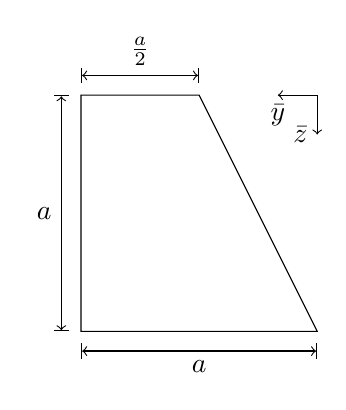
\begin{tikzpicture}
                \draw (0,0) -- (3,0) -- (1.5,3) -- (0,3) -- cycle;
                \draw[|<->|] (0,-.25) -- (3,-.25) node[midway,below] {\(a\)};
                \draw[|<->|] (-.25,0) -- (-.25,3) node[midway,left] {\(a\)};
                \draw[|<->|] (0,3.25) -- (1.5,3.25) node[midway,above] {\(\frac{a}{2}\)};
                \draw[->] (3,3) -- (2.5,3) node[below] {\(\bar{y}\)};
                \draw[->] (3,3) -- (3,2.5) node[left] {\(\bar{z}\)};
            \end{tikzpicture}
        \end{center}
        Gegeben: \(M = 2Fl\), \(F\), \(l\), \(a\)
    \end{problem}
    
    \subsection*{Lösung}
    Um die maximale Biegespannung zu bestimmen wird die Formel für die Biegespannung benötigt, welche sich auf das Hauptachsensystem bezieht.
    Somit muss zuerst dieses ermittelt werden.
    Anschließend muss der Punkt der höchsten Spannung und der dazugehörige Spannungswert ermittelt werden.
    Die maximale Spannnung ist der Punkt im Querschnitt, der am weitesten von der neutralen Linie entfernt ist.
    Insgesamt sind die folgenden Schritte notwendig:
    \begin{enumerate}[label=\arabic*)]
        \item \emph{Berechnung des Schwerpunktes des Balkenquerschnitts:} Die Aufteilung der Geometrie erfolgt in einem Quadrat der Kantenlänge \(a\) und ein negatives Dreieck.
        \begin{center}
            \begin{tabular}{lcccccc}
                \toprule
                \(i\) & \(A_i\) & \(\bar{y}_{s, i}A_i\) & \(\bar{z}_{s, i}\) & \(\bar{z}_{s, i}A_i\)\\
                \midrule
                \(I\) & \(a^2\) & \(\frac{a}{2}\) & \(\frac{a^3}{2}\) & \(\frac{a}{2}\) & \(\frac{a^3}{2}\)\\
                \(-II\) & \(\parentheses*{-}\frac{a^2}{4}\) & \(\frac{a}{6}\) & \(\parentheses*{-}\frac{a^3}{24}\) & \(\frac{a}{3}\) & \(\parentheses*{-}\frac{a^3}{12}\)\\
                \midrule
                \(\sum\) & \(\frac{3}{4}a^2\) & & \(\frac{11}{24}a^3\) & & \(\frac{5}{12}a^3\)\\
                \bottomrule
            \end{tabular}
        \end{center}
        \[
            \bar{y}_s = \frac{1}{A}\sum\bar{y}_{s, i}A_i = \frac{\frac{11}{24}a^3}{\frac{3}{4}a^2} = \frac{11}{18}a, \quad \bar{z}_s = \frac{1}{A}\sum\bar{z}_{s, i}A_i = \frac{\frac{5}{12}a^3}{\frac{3}{4}a^2} = \frac{5}{9}a.
        \]
        \item \emph{Berechnung der Flächenträgheitsmomente im Schwerpunktsystem:} Mit den Abkürzungen \(\Delta z_{s, i} = \bar{z}_{s, i} - \bar{z}_s\) und \(\Delta y_{s, i} = \bar{y}_{s, i} - \bar{y}_s\) folgt für die Flächenträgheitsmomente:
        \begin{center}
            \begin{tabular}{lcccccccc}
                \toprule
                \(i\) & \(I_{y, i}\) & \(\Delta z_{s, i}\) & \(\Delta z_{s, i}^2 A_i\) & \(I_{z, i}\) & \(\Delta y_{s, i}\) & \(\Delta y_{s, i}^2 A_i\) & \(I_{yz, i}\) & \(\Delta y_{s, i}\Delta z_{s, i}A_i\)\\
                \midrule
                \(I\) & \(\frac{a^4}{12}\) & \(-\frac{a}{18}\) & \(\frac{a^4}{324}\) & \(\frac{a^4}{12}\) & \(-\frac{a}{9}\) & \(\frac{a^4}{81}\) & \(0\) & \(\frac{a^4}{162}\)\\
                \(-II\) & \(\parentheses*{-}\frac{a^4}{72}\) & \(-\frac{2}{9}a\) & \(\parentheses*{-}\frac{a^4}{81}\) & \(\parentheses*{-}\frac{a^4}{288}\) & \(-\frac{4}{9}a\) & \(\parentheses*{-}\frac{4}{81}a^4\) & \(\parentheses*{-}\frac{a^4}{288}\) & \(\parentheses*{-}\frac{2}{81}a^4\)\\
                \midrule
                \(\sum\) & \(\frac{5}{72}a^4\) & & \(-\frac{a^4}{108}\) & \(\frac{23}{288}a^4\) & & \(-\frac{3}{81}a\) & \(-\frac{a^4}{288}\) & \(-\frac{a^4}{54}\)\\
                \bottomrule
            \end{tabular}
        \end{center}
        \begin{align*}
            I_y &= \sum I_{y, i} + \sum\parentheses*{\bar{z}_{s, i} - \bar{z}_s}^2 A_i = \frac{13}{216}a^4,\\
            I_z &= \sum I_{z, i} + \sum\parentheses*{\bar{y}_{s, i} - \bar{y}_s}^2 A_i = \frac{37}{864}a^4,\\
            I_{yz} &= \sum I_{yz, i} + \sum\parentheses*{\bar{y}_{s, i} - \bar{y}_s}\parentheses*{\bar{y}_{s, i} - \bar{z}_s} A_i = \frac{13}{864}a^4.
        \end{align*}
        \item \emph{Berechnunng der Hauptträgheitsmomente:} Da die Formel für die Biegespannung im Hauptachsensystem gilt, müssen auch die Flächenträgheitsmomente in diesem System berechnet werden.
        Die Hauptträgheitsmomente ergeben sich aus
        \[
            I_{1, 2} = \frac{I_y + I_z}{2} \pm \sqrt{\parentheses*{\frac{I_y - I_z}{2}}^2 + I_{yz}^2}
        \]
        und dies führt zu
        \[
            I_1 = 0,06888a^4, \quad I_2 = 0,03413a^4.
        \]
        \item \emph{Berechnung der Hauptachsen:} Aus
        \[
            \tan\parentheses*{2\varphi^*} = \frac{2I_{yz}}{I_y - I_z}
        \]
        ergibt sich
        \[
            \varphi^* = 30,009^\circ.
        \]
        Einsetzen in die Transformationsgleichungen liefert für das um \(30,009^\circ\) gedrehte Hauptachsensystem \(y'\)-\(z'\) demnach
        \[
            I_{y'} = I_1, \quad I_{z'} = I_2.
        \]
        \item \emph{Berechnung der angreifenden Momente:} Zur Bestimmung der Momentenrichtungen lässt sich die Rechte-Hand-Regel nutzen.
        Mit dieser ergeben sich die folgenden Momentenverläufe im ursprünglichen \(\bar{y}\)-\(\bar{z}\)-Koordinatensystem
        \[
            M_y\parentheses*{x} = F\parentheses*{x - l}, \quad M_z\parentheses*{x} = -M = -2Fl.
        \]
        Uns interessiert der Spannungszustand in der Mitte des Balkens
        \[
            M_y\parentheses*{x = \frac{l}{2}} = M_y = -\frac{Fl}{2}, \quad M_z\parentheses*{x = \frac{l}{2}} = M_z = -2Fl.
        \]
        Die Momente im Hauptachsensystem ergeben sich aus den Winkelbeziehungen wie folgt:
        \begin{align*}
            M_{y'}\parentheses*{x' = \frac{l}{2}} = M_{y'} = M_y\cos\varphi^* + M_z\sin\varphi^* = -1,4332Fl,\\
            M_{z'}\parentheses*{x' = \frac{l}{2}} = M_{z'} = -M_y\sin\varphi^* + M_z\cos\varphi^* = -1,4818Fl.
        \end{align*}
        \item \emph{Berechnung der Biegespannungsverteilung:} Aus den ermittelten Größen lässt sich nun die Formel für die Biegespannungsverteilung aufstellen:
        \[
            \sigma_b\parentheses*{y', z'} = \frac{M_{y'}}{I_{y'}}z' - \frac{M_{z'}}{I_{z'}}y' = \parentheses*{-20,8079z' + 43,4171y'}\frac{Fl}{a^4}.
        \]
        \item \emph{Bestimmung der neutralen Linie:} Aus der Bedingung für die neutrale Linie \(\sigma_b\parentheses*{y', z'} = 0\) folgt nach Auflösen nach \(y'\) die Geradengleichung
        \[
            y' = 0,4793z'.
        \]
        \item \emph{Ermittlung des am weitesten von der neutralen Linie entfernten Punkt:} Maximale Biegespannungen treten am Punkt \(A\) auf, da dieser am weitesten von der neutralen Linie entfernt liegt.
        Der Punkt hat im ursprünglichen \(\bar{y}\)-\(\bar{z}\)-Koordinatensystem die Koordinaten \(\parentheses*{0, a}\).
        Im \(y\)-\(z\)-Schwerpunktkoordinatensystem hat er somit die Koordinaten
        \[
            \parentheses*{y_A, z_A} = \parentheses*{0 - \bar{z}_s, a - \bar{z}_s} = \parentheses*{-\frac{11}{18}a, \frac{4}{9}a}.
        \]
        Die \(y'\)-\(z'\)-Koordinaten im Hauptachsensystem des Punktes \(A\) berechnen sich mithilfe einer Drehmatrix zu
        \[
            \begin{pmatrix}
                y_A'\\
                z_A'
            \end{pmatrix} = \begin{pmatrix}
                \cos\varphi^* & \sin\varphi^*\\
                -\sin\varphi^* & \cos\varphi^*
            \end{pmatrix}\begin{pmatrix}
                y_A\\
                z_A
            \end{pmatrix} = \begin{pmatrix}
                -0,3069a\\
                0,6905a
            \end{pmatrix}.
        \]
        \item \emph{Bestimmung der maximalen Biegespannung:} Für die betragsmäßig maximale Biegespannung ergibt sich folglich
        \[
            \sigma_b\parentheses*{-0,3069a, 0,6905a} = -27,693\frac{Fl}{a^4}.
        \]
    \end{enumerate}


    \section*{Aufgabe 2}
    
    \begin{problem}
        Ein Balken mit L-Profil ist an der Stelle \(A\) fest eingespannt und wird wie gezeigt durch ein Moment \(M\) belastet.
        Berechnen Sie
        \begin{enumerate}
            \item den Schwerpunkt des Balkenquerschnitts,
            \item die Flächenträgheitsmomente im Schwerpunktsystem,
            \item die Hauptträgheitsmomente,
            \item die Hauptachsen,
            \item die Biegespannungsverteilung,
            \item die neutrale Linie und
            \item die maximale Biegespannung.
        \end{enumerate}
        \begin{center}
            \begin{tikzpicture}
                \draw[very thick] (0,0) node[above right] {\(A\)} -- (3,0);
                \draw[->] (3,0) -- (3.5,0) node[right] {\(x\)};
                \draw[->] (0,-1) -- (0,1.5) node[above] {\(y\)};
                \draw[->] (2.8,.2) arc (135:-135:.3cm);
                \node[anchor=north east] at (2.8,-.2) {\(M\)};
            \end{tikzpicture}
            \quad
            \begin{tikzpicture}
                \draw (0,0) -- (0,4) -- (.5,4) -- (.5,1) -- (2,1) -- (2,0) -- cycle;
                \draw[|<->] (-.25,0) -- (-.25,1) node[midway,left] {\(h_2\)};
                \draw[<->|] (-.25,1) -- (-.25,4) node[midway,left] {\(h_1\)};
                \draw[|<->] (0,4.25) -- (.5,4.25) node[midway,above] {\(b_1\)};
                \draw[|<->|] (0,-.25) -- (2,-.25) node[midway,below] {\(b_2\)};
                \draw[->] (.5,4) -- (.5,4.75) node[above] {\(\bar{y}\)};
                \draw[->] (0,1) -- (-.75,1) node[left] {\(\bar{z}\)};
            \end{tikzpicture}
        \end{center}
        Gegeben: \(b_1 = 1\sis{\centi\meter}\), \(b_2 = 4\sis{\centi\meter}\), \(h_1 = 6\sis{\centi\meter}\), \(h_2 = 2\sis{\centi\meter}\), \(M = 100\sis{\newton\meter}\)
    \end{problem}
    
    \subsection*{Lösung}
    \begin{enumerate}
        \item\,
        \begin{center}
            \begin{tabular}{lcccccc}
                \toprule
                \(i\) & \(A_i\) & \(\bar{y}_{s, i}A_i\) & \(\bar{z}_{s, i}\) & \(\bar{z}_{s, i}A_i\)\\
                \midrule
                \(I\) & \(6\sis{\centi\meter\squared}\) & \(3\sis{\centi\meter}\) & \(18\sis{\centi\meter\cubed}\) & \(0,5\sis{\centi\meter}\) & \(3\sis{\centi\meter\cubed}\)\\
                \(II\) & \(8\sis{\centi\meter\squared}\) & \(-1\sis{\centi\meter}\) & \(-8\sis{\centi\meter\cubed}\) & \(-1\sis{\centi\meter}\) & \(-8\sis{\centi\meter\cubed}\)\\
                \midrule
                \(\sum\) & \(14\sis{\centi\meter\squared}\) & & \(10\sis{\centi\meter\cubed}\) & & \(-5\sis{\centi\meter\cubed}\)\\
                \bottomrule
            \end{tabular}
        \end{center}
        \[
            \bar{y}_s = \frac{1}{A}\sum\bar{y}_{s, i}A_i = \frac{10\sis{\centi\meter\cubed}}{14\sis{\centi\meter\squared}} = \frac{5}{7}\sis{\centi\meter}, \quad \bar{z}_s = \frac{1}{A}\sum\bar{z}_{s, i}A_i = -\frac{5\sis{\centi\meter\cubed}}{14\sis{\centi\meter\squared}} = -\frac{5}{14}\sis{\centi\meter}.
        \]
        \item Mit den Abkürzungen \(\Delta z_{s, i} = \bar{z}_{s, i} - \bar{z}_s\) und \(\Delta y_{s, i} = \bar{y}_{s, i} - \bar{y}_s\) folgt für die Flächenträgheitsmomente:
        \begin{center}
            \begin{tabular}{lcccccccc}
                \toprule
                \(i\) & \(I_{y, i}\) & \(\Delta z_{s, i}\) & \(\Delta z_{s, i}^2 A_i\) & \(I_{z, i}\) & \(\Delta y_{s, i}\) & \(\Delta y_{s, i}^2 A_i\) & \(I_{yz, i}\) & \(\Delta y_{s, i}\Delta z_{s, i}A_i\)\\
                \midrule
                \(I\) & \(0,5\sis{\centi\meter\tothe{4}}\) & \(\frac{6}{7}\sis{\centi\meter}\) & \(\frac{216}{49}\sis{\centi\meter\tothe{4}}\) & \(18\sis{\centi\meter\tothe{4}}\) & \(\frac{16}{7}\sis{\centi\meter}\) & \(\frac{1536}{49}\sis{\centi\meter\tothe{4}}\) & \(0\sis{\centi\meter\tothe{4}}\) & \(\frac{576}{49}\sis{\centi\meter\tothe{4}}\)\\
                \(II\) & \(\frac{32}{3}\sis{\centi\meter\tothe{4}}\) & \(-\frac{9}{14}\sis{\centi\meter}\) & \(\frac{162}{49}\sis{\centi\meter\tothe{4}}\) & \(\frac{8}{3}\sis{\centi\meter\tothe{4}}\) & \(-\frac{12}{7}\sis{\centi\meter}\) & \(\frac{1152}{49}\sis{\centi\meter\tothe{4}}\) & \(0\sis{\centi\meter\tothe{4}}\) & \(\frac{432}{49}\sis{\centi\meter\tothe{4}}\)\\
                \midrule
                \(\sum\) & \(\frac{32}{3}\sis{\centi\meter\tothe{4}}\) & & \(\frac{54}{7}\sis{\centi\meter\tothe{4}}\) & \(\frac{62}{3}\sis{\centi\meter\tothe{4}}\) &  & \(\frac{384}{7}\sis{\centi\meter\tothe{4}}\) & \(0\sis{\centi\meter\tothe{4}}\) & \(\frac{144}{7}\sis{\centi\meter\tothe{4}}\)\\
                \bottomrule
            \end{tabular}
        \end{center}
        \begin{align*}
            I_y &= \sum I_{y, i} + \sum\parentheses*{\bar{z}_{s, i} - \bar{z}_s}^2 A_i = 18\frac{37}{42}\sis{\centi\meter\tothe{4}},\\
            I_z &= \sum I_{z, i} + \sum\parentheses*{\bar{y}_{s, i} - \bar{y}_s}^2 A_i = 75\frac{11}{21}\sis{\centi\meter\tothe{4}},\\
            I_{yz} &= \sum I_{yz, i} + \sum\parentheses*{\bar{y}_{s, i} - \bar{y}_s}\parentheses*{\bar{y}_{s, i} - \bar{z}_s} A_i = -20\frac{4}{7}\sis{\centi\meter\tothe{4}}.
        \end{align*}
        \item
        \[
            I_{1, 2} = \frac{I_y + I_z}{2} \pm \sqrt{\parentheses*{\frac{I_y + I_z}{2}}^2 + I_{yz}^2}
        \]
        führt zu
        \[
            I_1 = 82,206\sis{\centi\meter\tothe{4}}, \quad I_2 = 12,198\sis{\centi\meter\tothe{4}}.
        \]
        \item Aus
        \[
            \tan\parentheses*{2\varphi^*} = \frac{2I_{yz}}{I_y - I_z}
        \]
        ergibt sich
        \[
            \varphi^* = 17,996^\circ.
        \]
        Einsetzen in die Transformationsgleichungen liefert \(\varphi_2^* = 17,996^\circ\).
        Im Hauptachsensystem \(y'\)-\(z'\) gilt demnach
        \[
            I_{y'} = 12,198\sis{\centi\meter\tothe{4}}, \quad I_{z'} = 82,206\sis{\centi\meter\tothe{4}}.
        \]
        \item Für die Biegespannungsverteilung muss das Biegemoment in Komponenten entlang der Hauptachsen zerlegt werden (Rechte-Hand-Regel):
        \[
            M_{y'} = -M\sin\varphi^* = -30,895\sis{\newton\meter}, \quad M_{z'} = -M\cos\varphi^* = -95,108\sis{\newton\meter}.
        \]
        Setzt man dies in die Biegespannung ein, folgt folgende Gleichung
        \[
            \sigma_b\parentheses*{y', z'} = \frac{M_{y'}}{I_{y'}}z' - \frac{M_{z'}}{I_{z'}}y' = -253,28\sis{\newton\per\centi\meter\cubed}z' + 115,694\sis{\newton\per\centi\meter\cubed}y'.
        \]
        \item Aus der Bedingung für die neutrale Linie \(\sigma_b\parentheses*{y', z'} = 0\) folgt nach Auflösen nach \(y'\) die Geradengleichung
        \[
            y' = 2,189z'.
        \]
        \item Maximale Biegespannungen treten am Punkt \(A\) auf, da dieser am weitesten von der neutralen Linie entfernt liegt.
        Der Punkt hat im ursprünglichen \(\bar{y}\)-\(\bar{z}\)-Koordinatensystem die Koordinaten \(\parentheses*{6\sis{\centi\meter}, 0\sis{\centi\meter}}\).
        Im \(y\)-\(z\)-Schwerpunktkoordinatensystem hat er somit die Koordinaten \(\parentheses*{5\frac{2}{7}\sis{\centi\meter}, \frac{5}{14}\sis{\centi\meter}}\).
        Die \(y'\)-\(z'\)-Koordinaten im Hauptachsensystem des Punktes \(A\) berechnen sich mithilfe einer Drehmatrix zu
        \[
            \begin{pmatrix}
                y_A'\\
                z_A'
            \end{pmatrix} = \begin{pmatrix}
                \cos\varphi^* & \sin\varphi^*\\
                -\sin\varphi^* & \cos\varphi^*
            \end{pmatrix}\begin{pmatrix}
                y_A\\
                z_A
            \end{pmatrix} = \begin{pmatrix}
                5,137\sis{\centi\meter}\\
                -1,293\sis{\centi\meter}
            \end{pmatrix}.
        \]
        Für die maximale Biegespannung ergibt sich folglich
        \[
            \sigma_b\parentheses*{5,137\sis{\centi\meter}, -1,293\sis{\centi\meter}} = 921,811\sis{\newton\per\centi\meter\squared}.
        \]
    \end{enumerate}
\end{document}
